\documentclass[11pt]{standalone}
\usepackage[utf8]{inputenc}
\usepackage{amsmath}
\usepackage{amsfonts}
\usepackage{amssymb}
\usepackage{tikz}
\usepackage{pgfplots}
\pgfplotsset{compat=1.3}
\begin{document}


%%%%%%%%%%%% ht-grafiek %%%%%%%%%%%%%%%%%%%%%
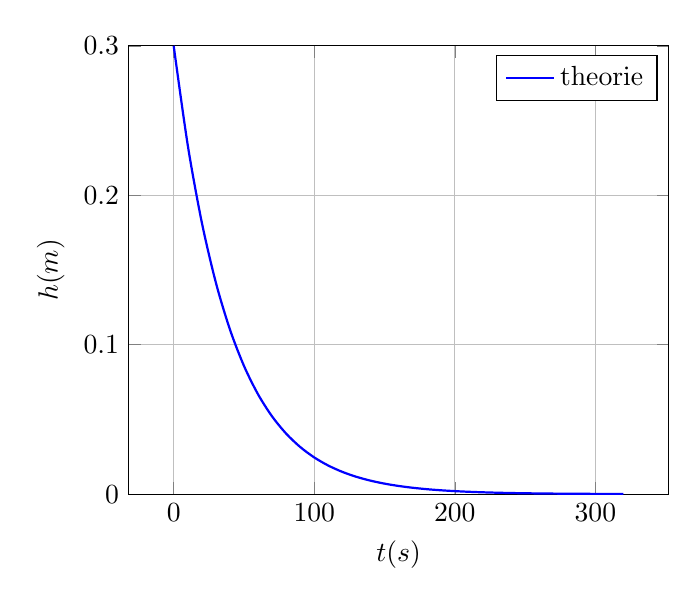
\begin{tikzpicture}
\begin{axis}[
    xlabel = $t(s)$,
    ylabel = {$h(m)$},
    ymax=0.3,
    ymin=0,
    grid=both,
]
%Below the red parabola is defined
\addplot [smooth,
    domain=0:300, 
    samples=100, 
    thick,
    color=blue,
]
coordinates {(0,0.30)(10,0.233567112)(20,0.181845319)(30,0.141576953)(40,0.110225734)(50,0.085817021)(60,0.066813446)(70,0.052018079)(80,0.040499041)(90,0.031530814)(100,0.024548537)(110,0.019112436)(120,0.014880122)(130,0.011585024)(140,0.009019602)(150,0.007022274)(160,0.005467241)(170,0.004256559)(180,0.003313974)(190,0.002580118)(200,0.002008769)(210,0.001563941)(220,0.001217617)(230,0.000947985)(240,0.00073806)(250,0.000574622)(260,0.000447376)(270,0.000348308)(280,0.000271177)(290,0.000211127)(300,0.000164374)(310,0.000127975)(319.9,9.98855E-05)};
\addlegendentry{theorie}
\end{axis}
\end{tikzpicture}

%%%%%%%%%%%%%%%%%%%% v(h) t-grafiek %%%%%%%%%%%%%%%%
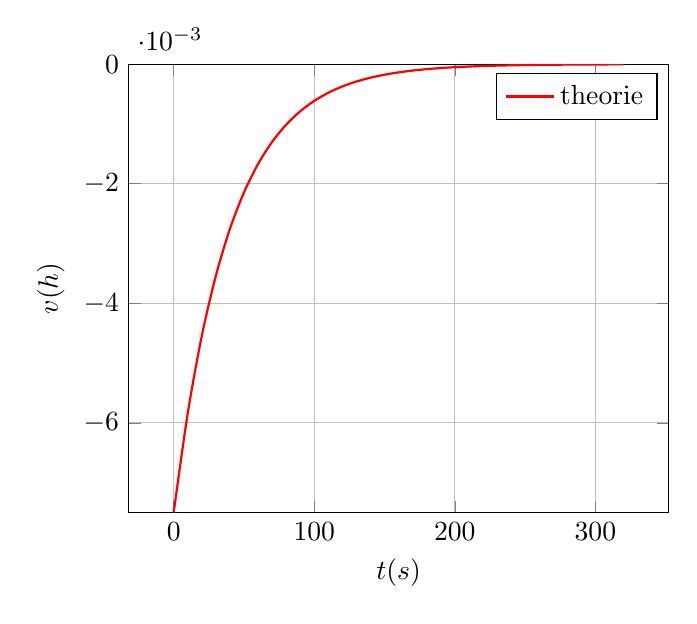
\begin{tikzpicture}
\begin{axis}[
    xlabel = $t(s)$,
    ylabel = {$v(h)$},
    ymax=0,
    ymin=-0.0075,	
    grid=both,
    anchor=north,
]
%Below the red parabola is defined
\addplot [smooth,
    domain=0:300, 
    samples=50, 
    thick,
    color=red,
]
coordinates {(0,-0.0075)(10,-0.005839178)(20,-0.004546133)(30,-0.003539424)(40,-0.002755643)(50,-0.002145426)(60,-0.001670336)(70,-0.001300452)(80,-0.001012476)(90,-0.00078827
)(100,-0.000613713)(110,-0.000477811)(120,-0.000372003)(130,-0.000289626
)(140,-0.00022549
)(150,-0.000175557
)(160,-0.000136681
)(170,-0.000106414
)(180,-8.28494E-05
)(190,-6.45029E-05
)(200,-5.02192E-05
)(210,-3.90985E-05
)(220,-3.04404E-05
)(230,-0.00002369961487127)(240,-0.00001845150199359)(250,-0.00001436554676812)(260,-0.00001118439756387)(270,-0.00000870769145692)(280,-0.00000677943448236)(290,-5.27818E-06)(300,-0.00000410936142409)(310,-0.00000319937226494)(319.9,-0.00000249713664074)};
\addlegendentry{theorie}
\end{axis}
\end{tikzpicture}
\end{document}